%
% $Id: FIR.tex 14 2014-02-04 22:36:30Z nicb $
%

\section{Un filtro FIR semplice\label{sec:simple fir}}

\subsection{Dominio continuo di tempo\label{sec:continuous time}}

Nei filtri FIR (\emph{feed-forward}) l'output \`e la somma dell'input e una versione riscalata e ritardata
		dell'input:

		\begin{equation}\label{eqn:fir semplice}
						y_t = x_t + a_1 x_{t-\tau}
			\end{equation}

		(aggiungere grafico)

	Poniamo che $x_t$ sia un segnale sinusoidale complesso:

		 \begin{equation}
	    x_t = e^{i\omega t}\nonumber
		 \end{equation}

		 \begin{equation}
			y_t = e^{i \omega t} + a_1 e^{i \omega (t - \tau)}
		 \end{equation}

		(fare schemino sul cerchio unitario)

		 \begin{equation}
		  y_t = e^{i \omega t} + a_1 e^{i \omega t} e^{-i \omega \tau} = e^{i\omega t} \left [ 1 + a_1 e^{-i \omega \tau} \right ]
		 \end{equation}

	Quindi l'uscita \`e sempre un fasore di frequenza $\omega$ moltiplicato per
		un'ampiezza che \`e funzione di $\omega$ (ma indipendente dal tempo!)

	La funzione del filtro \`e dunque $\left [ 1 + a_1 e^{-i \omega \tau} \right ]$ e la chiameremo $H(\omega)$

	Per capire la risposta in frequenza e in fase dobbiamo capire che $H(\omega)$ \`e
		in realt\`a la magnitudine (valore assoluto di $H(\omega)$ moltiplicata per una
		funzione della fase:

		 \begin{equation}
		  H(\omega) = |H(\omega)| e^{i \Theta(\omega)}
		 \end{equation}

	 dove $|H(\omega)| = |1 + a_1 e^{-i\omega \tau}|$; siccome per il teorema di Pitagora il
	 modulo \`e il quadrato della parte reale + il quadrato della parte
	 immaginaria sotto radice,

		 \begin{equation}
	  Re(H(\omega)) = 1 + a_1 cos(\omega \tau)
		 \end{equation}
		 \begin{equation}
		Im(H(\omega)) = - a_1 sin(\omega \tau)
		 \end{equation}

		 \begin{equation}
	  Re^2 = 1 + 2 a_1 cos(\omega \tau) + a_1^2 cos^2(\omega \tau)
		 \end{equation}
		 \begin{equation}
		Im^2 = a_1^2 sin^2(\omega \tau)
		 \end{equation}

		quindi
		
		 \begin{equation}
		Re^2 + Im^2 = 1 + 2 a_1 cos(\omega \tau) + a^2 [ cos^2(\omega \tau) + sin^2(\omega \tau) ]
		 \end{equation}

		 Dato che

		 \begin{equation}
				cos^2(\alpha) + sin^2(\alpha) = 1
		 \end{equation}

		 per $\alpha$ qualsiasi,

		 \begin{equation}
				1 + 2 a_1 cos(\omega \tau) + a^2 [ cos^2(\omega \tau) + sin^2(\omega \tau) ] = 1 + 2 a_1 cos(\omega \tau) + a^2
		 \end{equation}
		 \begin{figure}[htb]
			 \begin{center}
					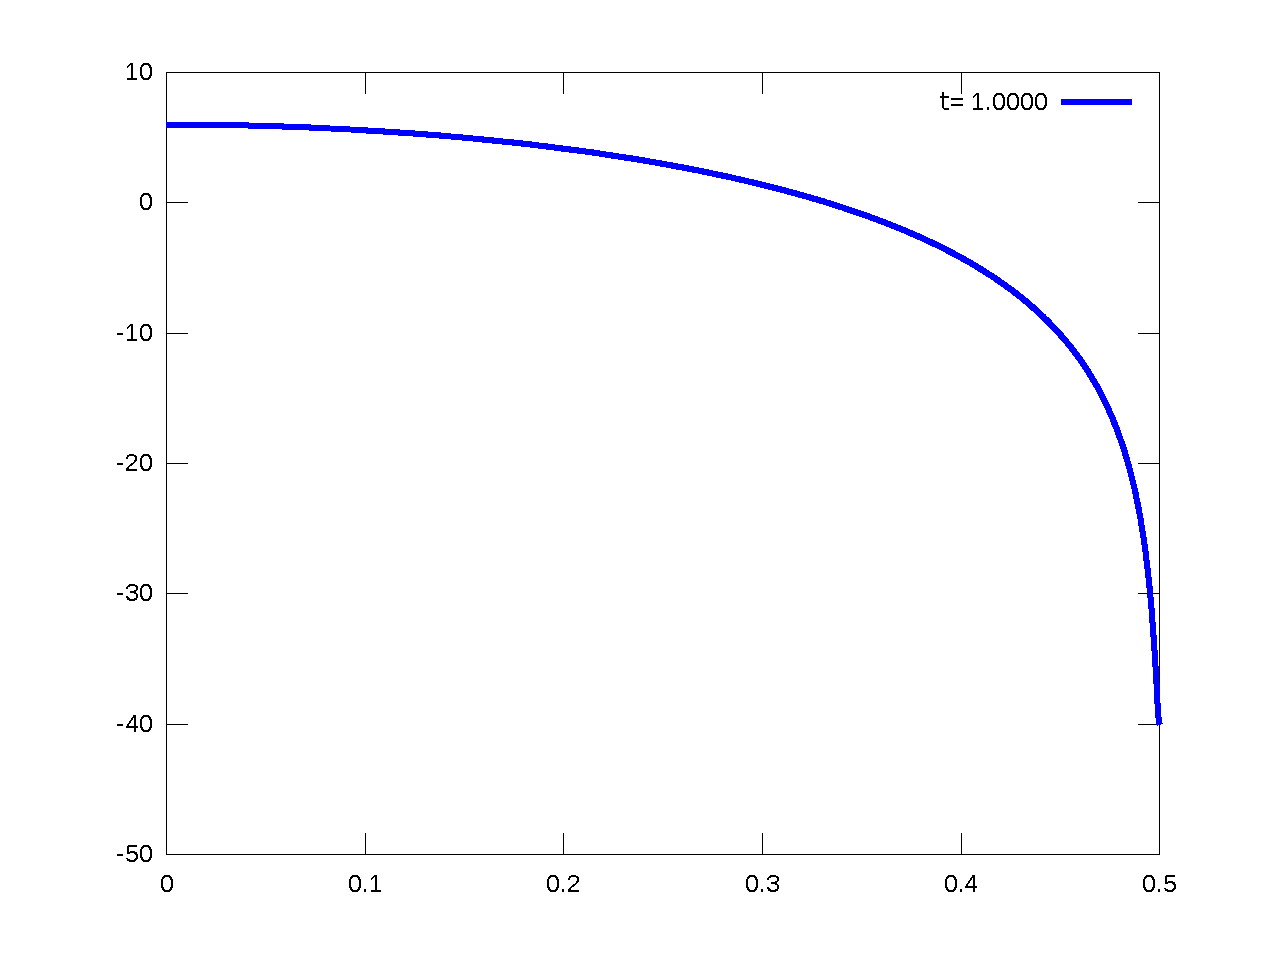
\includegraphics[width=0.8\textwidth]{\plotdir/fir2}
					\caption{Filtro FIR con $\tau = 1/fc$\label{fig:fir con tau 1}}
			 \end{center}
		 \end{figure}
		 \begin{figure}[htb]
			 \begin{center}
					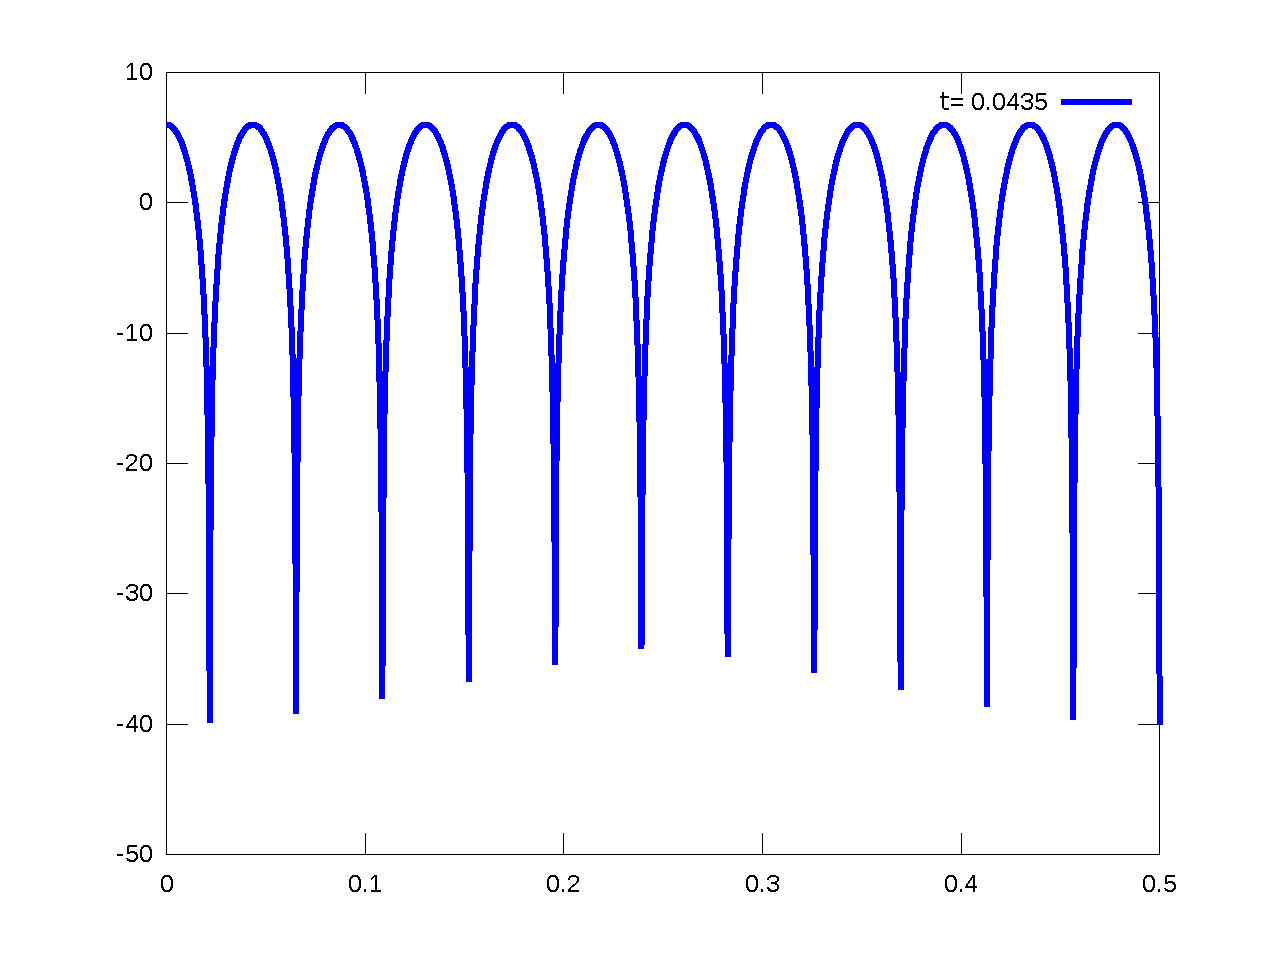
\includegraphics[width=0.8\textwidth]{\plotdir/fir3}
					\caption{Filtro FIR con $\tau = 23/fc$\label{fig:fir con tau 23}}
			 \end{center}
		 \end{figure}
		 Le Figg.\vref{fig:fir con tau 1} e \vref{fig:fir con tau 23} mostrano la
		 risposta in frequenza rispettivamente per $\tau = 1/fc$ e per $\tau = 23/fc$.

\subsection{Esercizi}

\begin{itemize}

	\item fare il plot della risposta in frequenza con vari valori di $\omega$ e
					di $\tau$

\end{itemize}


\subsection{Passaggio dal tempo continuo al tempo discreto}


	Il ritardo $\tau$ viene ristretto ad un numero intero di campioni multiplo della
		periodo di campionamento $T_s$ (restrizione)

	Dato che la frequenza di campionamento interesser\`a  la  definizione
    del  nostro  segnale  (per  le  frequenze  che   servono   per   una
    applicazione piuttosto che un'altra), ma non  il  funzionamento  del
    filtro, possiamo  benissimo  normalizzare  la  nostra  frequenza  di
    campionamento a $1$, avendo cos\`i la frequenza di Nyquist a $0.5$

	Ora, se noi ritardiamo il nostro segnale di un campione (invece che del
		valore continuo tau) moltiplicheremo il nostro fasore in ingresso per
		$e^{-i \omega T}$ dove $\omega T$ \`e l'angolo in radianti per campione. Possiamo sempre
		ricavare il tempo nel dominio digitale moltiplicando per il periodo di
		campionamento $T_s$ - possiamo quindi evitare di scrivere $T_s$, che diventa
		una sorta di costante di conversione: se la costante \`e 1 (frq di
		campionamento 1) possiamo evitare di scriverla ogni volta

	La frequenza di campionamento diventa $\omega = 2 \pi$ e la frequenza di nyquist \`e
		$\omega = \pi$ radianti per campione e il nostro fasore sar\`a sempre

		 \begin{equation}
	 			x_t = e^{i\omega kT}
		 \end{equation}
		
		dove $k$ \`e un numero intero di campioni e $T$ \`e il periodo di campionamento

		Ora rifacciamo il filtro dell'eq.\ref{eqn:fir semplice} della Sez.\vref{sec:continuous time} ritardando per\`o non di tau
	  ma di un solo campione:

		 \begin{equation}
		   y_k = x_k + a_1 x_{k-1}
		 \end{equation}

	  applicando il fasore digitale, il filtro diventer\`a:

		 \begin{equation}
	  	  y_k = e^{i\omega kT} [ 1 + a_1 e^{-i\omega \times 1} ] = e^{i \omega kT} [ 1 + a_1 e^{-i \omega } ]
		 \end{equation}

		e la magnitudine (== risposta in frequenza) sar\`a:

		 \begin{equation}
		  |H( \omega )| = 1 + 2 a_1 cos( \omega ) + a_1^2
		 \end{equation}

	Ricapitolando, se l'input di un filtro FIR \`e il fasore $e^{i \omega kT}$

		 \begin{equation}
	   y_t = a_0 x_t + a_1 x_{t-1}
		 \end{equation}

    (ritardo di un campione).

		L'output \`e anche un fasore con frequenze inalterate

		 \begin{equation}
		 y_k = x_k \left [ a_0 + a_1 e^{-i \omega} \right ]
		 \end{equation}

		possiamo aggiungere quanti termini vogliamo in un filtro del genere:

		 \begin{equation}
		 y_k = x_k \left [ a_0 + a_1 e^{-i\omega } + a_2 e^{-i2\omega } + a_3 e^{-i3\omega } + ... + a_n e^{-in\omega } \right ]
		 \end{equation}


	Invece di ripetere $e^{i\omega}$ ogni volta, possiamo operare una sostituzione: sostituiamo $z = e^{i \omega}$

	Il ritardo di un campione diventa cos\`i $z^{-1}$, e il ritardo di $k$ campioni
		diventa cos\`i $z^{-k}$

	$z^{-1}$ \`e trattabile sia come una variabile complessa che come un
		operatore, cio\`e una operazione applicata ad un certo oggetto (pensate
		p.es. ad un operatore che ruota un disegno di 90 gradi) $= \rho$: $\rho^2$ lo
		ruota di 180 gradi in senso antiorario, $\rho^{-1}$ lo ruota in senso orario)

	Possiamo anche usare la notazione $X$ per rappresentare un \emph{intero segnale}
		(un vettore di campioni); nota bene: $x_k$ rappresenta il valore di un
		segnale al tempo $k$, $X$ rappresenta \emph{l'intero segnale}.

	L'intero segnale ritardato di un campione \`e quindi notato $z^{-1} X$ quindi
		significa ``applica l'operatore $z^{-1}$ al segnale $X$''

		L'equazione si riscrive:

		 \begin{equation}
		  Y = a_0 X + a_1 z^{-1} X = \left [ a_0 + a_1 z^{-1} \right ] X
		 \end{equation}

		(nota che anche l'ampiezza diventa un operatore: moltiplica \emph{tutto il
		segnale} per la costante $a_0$, e quest'operatore \`e commutativo).

	Quindi $Y = H(z) X$ dove $H(z) = a_0 + a_1 z^{-1}$.

% \item se del caso fare due filtri in cascata moltiplicando le funzioni di
% 	trasferimento

\subsection{Esercizi}

\begin{enumerate}

	\item Si descriva un filtro FIR con l'equazione che segue:

					\begin{equation}
						y_k = x_k + x_{k-1} + x_{k-2} + \ldots + x_{k-19}
					\end{equation}

				Si derivi una espressione algebrica semplice per la sua risposta in
				magnitudine. Si trovi quali siano le frequenze alle quali si trovano
				dei picchi e quelle alle quali si trovano dei buchi

\end{enumerate}
